\documentclass{article}
\usepackage[utf8]{inputenc}
\usepackage{graphicx}

\title{Operating Systems Notes}
\author{Jacob Burley} %add your name here if you're a collaborator
\date{12 December 2017}

\begin{document}
%images aren't working for whatever reason (pdflatex doesn't find them at build time) which I think requires some extra configuration but the images aren't as important as the content so that's not a focus for me at the moment

\maketitle
\section{Introduction}
Operating System runs in kernel mode (supervisor mode), User programs run in User Mode
\\Instructions that control the machine or use I/O aren't available to User Mode (at least not directly)
%\\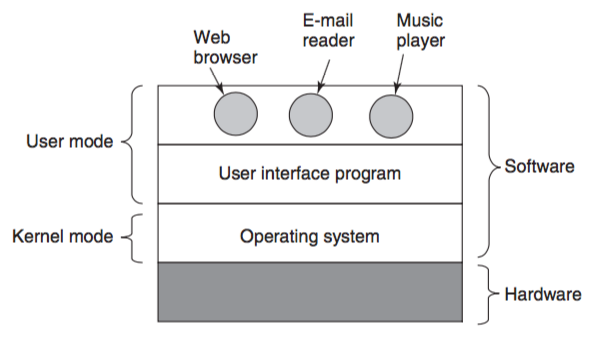
\includegraphics[width= 250pt]{tex/ch1/1-1.png}
\\Operating System runs on bare hardware
\\OS extends hardware of a computer, and makes it easier for programmers to develop applications without having to deal with things like SATA interfaces directly
\\OS also provides abstractions for devices, files etc.
%\\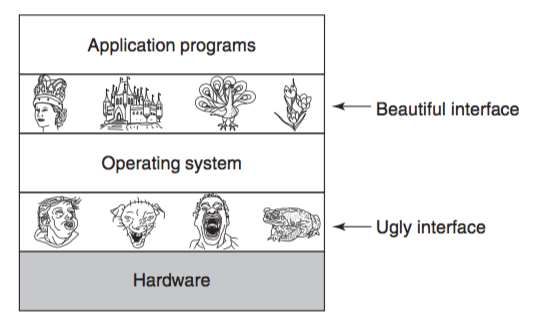
\includegraphics[width = 250pt]{tex/ch1/1-2.png}
\\OS also manages hardware resources like CPU and RAM, as well as I/O
\subsection*{First Generation Computers}
\\Earliest (first generation) computers didn't have an OS, were manually programmable using absolute machine language or physically rewiring plugboards to control basic functions of the machine
\subsection*{Second Generation Computers}
\\used transistors, became much more reliable
\\Batch systems involved collecting jobs on punchcards, reading them onto magnetic tape using a dedicated machine for this purpose, using this magnetic tape as input on the main computing machine, and then taking the output tape of that machine to another dedicated machine that printed the contents of the output tape
\\Structure of input job
\begin{itemize}
	\item \$JOB card, specifies maximum runtime in minutes, account number to be charged and programmer name
	\item \$FORTRAN card tells machine to load the FORTRAN compiler from the system tape, directly followed by program to be compiled
	\item \$LOAD card directed machine to load the object program that was just compiled
	\item \$RUN card, telling machine to run the program with the data that followed (like run-time arguments)
	\item \$END card marks the end of a job
\end{itemize}
\\used mostly for scientific and engineering calculations
\\They were largely programmed in FORTRAN and assembly
\\Typical OSes were the FORTRAN Monitor System, and IBM's IBSYS
\subsection*{Third Generation Computers}
\\Prior to 3rd gen, there were both large scale, word-oriented scientific computers but also character-oriented commercial computers
\section{Processes and Threads}

\section{Memory Management}

\section{File Systems}

\section{I/O}

\section{Deadlocks}
\\Systems have lots of resources that can only be used by one process at a time
\\We can't allow multiple processes to access a resource like a printer because it will lead to gibberish being printed
\\As a result, we allow a single process at a time to use resources like this
\\If process A requests a resource 1, and process B requests a resource 2, they are both granted these resources. If process A then requests resource 2 at the same time that process B requests resource 1, there will be a deadlock. Neither process will give up their currently held resource until they hold their newly requested resource, which means that neither process can advance.
\\
\\We have two types of resources: \textbf{preemptable}, and \textbf{Non-premptable}
\\\textbf{Preemptable} resources can be taken away from a process and given to another process without any ill effects. An example of this would be memory, as if a new process needs memory that an existing process occupies, then the memory that the existing process is using can simply be swapped out to disk, and the new process can take its place.
\\\textbf{Non-premptable} resources cannot be taken away from its current owner without potentially causing a failure. A device like a printer or a disk drive are examples of non-premptable resources
\\\textbf{non-premptable resources} are generally involved in deadlocks
\\deadlocks involving \textbf{preemptable resources} can usually be solved by reallocating resources
\\We assume that the sequence of events that all processes follow to use a resource is as follows
\begin{enumerate}
	\item Request the resource
	\item Use the resource
	\item Release the resource
\end{enumerate}
\\If a resource is not available on request, process may have to wait, may be blocked until it is available (depending on OS), or may receive an error code, in which case it can try again
\\Some kinds of resources (such as entries in a database) may be managed by the user processes themselves instead of the system, using semaphores or mutexes
\begin{lstlisting}[language=C]
/*
 * Using a semaphore to protect a single resource
 */
typedef int semaphore;
semaphore resource_1;

void process_A(void){
	down(&resource_1);
	use_resource_1();
	up(&resource_1);
}

/*
 * Using a semaphore to protect two resources
 */
typedef int semaphore;
semaphore resource_1;
semaphore resource_2;

void process_A(void){
	down(&resource_1);
	down(&resource_2);
	use_both_resources();
	up(&resource_2);
	up(&resource_1)
}
\end{lstlisting}
\\\textbf{Deadlock Definition:} \textit{A set of processes is deadlocked if each process in the set is waiting for an event that only another process in the set can cause.} 
\\4 conditions that must be present for resource deadlock to occur
\\each of these conditions represent a policy that may or may not be a characteristic of a given system
\\if one of the below is not present, no resource deadlock is possible
\begin{enumerate}
	\item Mutual exclusion condition: each resource is either currently assigned to exactly one process, or is available
	\item Hold-and-wait condition: processes currently holding resources that were granted earlier can request new resources
	\item No-preemption condition: Resources previously granted cannot be forcibly taken away from a process. They must be explicitly released by the process holding them
	\item Circular wait condition: There must be a circular list of two or more processes, each of which is waiting for a resource held by the next member of the chain
\end{enumerate}

\end{document}